\documentclass{article}
\usepackage{graphicx}

\begin{document}

\begin{titlepage}
\title{ECS189G Term Project Report Problem B}
\author{Goh Chang Kang, Charles 916751838 ccgoh@ucdavis.edu, \\
Yang Minxing 916751773 mixyang@ucdavis.edu, \\ 
Chen Jieyi Chloe 999823783 eyichen@ucdavis.edu}

\date{December 8, 2018}
\maketitle
\end{titlepage}

\tableofcontents

\pagebreak

\section{Introduction}

This dataset contains the following information: the drug’s name and condition, 
the patient’s review and rating, the review’s date and the number of users 
who found the review useful. 75\% of the data are in the training set and 
25\% are in the test set. The goal of the project is to investigate how 
reliable the verbal reviews are in establishing a numeric rating and predict 
the numeric rating using the verbal reviews and other useful variable 
information. We want to apply our model to predict ratings for other 
datasets that do not have numeric evaluation. We have 161297 number of 
observations in the training set and 53766 number of observations in the 
test set. Due to the limited computing power, we decide to randomly select 
12000 number of observations from the training set and 4000 from the test 
set to preserve the original train-test split ratio and minimize the 
dataset’s size while ensuring it is representative. 

\section{Obstacles}
In the general recommender system, we have user ID, item ID and rating. 
However, since this dataset was obtained by crawling online review sites, 
we do not know which individual rates the drug. In this case, the userID 
is unique for each review and it will affect the result from the Latent 
Factor Model because it takes user i’s effect on rating into consideration. 
Therefore, in order to provide a more accurate model, we decide to use the 
condition (disease that the drug cures) as userID because each 
condition/disease corresponds to multiple drug names. This modification 
can help us to create a more suitable data structure for the recommender 
system model.


\section{Data Pre-Processing}
\begin{itemize}
  \item Check whether there are missing values in the data
  \item Check the rating score distribution to see whether there is bias in the dataset
  \item Check whether the training set and test set have similar rating distribution
\end{itemize}

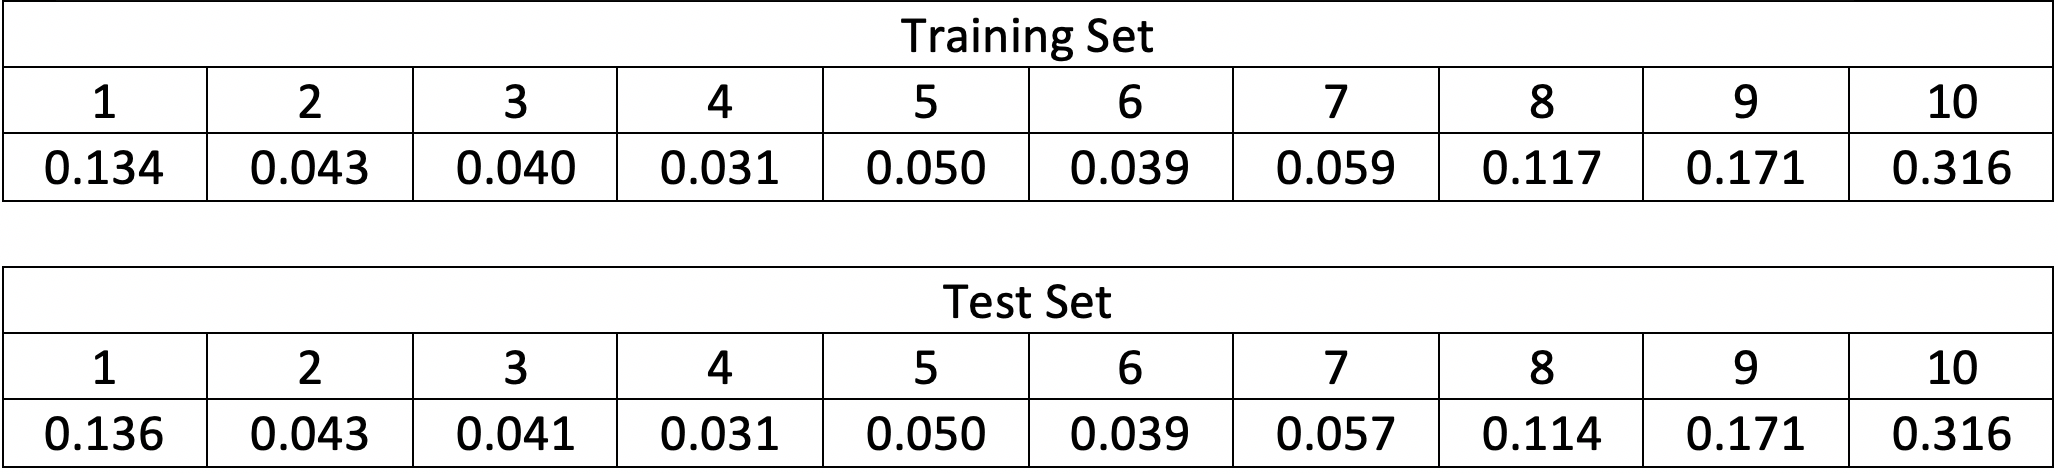
\includegraphics[scale=0.33]{data_preprocessing_problemB.png}
\newline
From the table above, we see that the training set and test set have very 
similar distribution. Both of them have relatively high number of ratings 
in score 10. 

\section{Review Data Pre-Processing for R Sentiment Analysis}
\begin{itemize}
  \item Tokenize the words, remove numbers, punctuations, symbols and hyphen
  \item Filter out the stop words (common words that provides very little meaning, such as 'the', 'a' and etc.)
  \item Perform stemming, in which takes similar words and collapse them into one on the tokens
  \item Save the processed tokens in a list
\end{itemize}


\section{Methods and Discussion}
We use R sentiment library (sentimentr) to analyze the feelings of the 
review response and get a numeric value (the average of the all the tokens’ 
sentiment score in a review) to indicate how positive or negative the 
review is. With the R sentiment analysis score, we find that some of the 
review scores tend to be negative even though the rating is relatively 
high. 
\newline
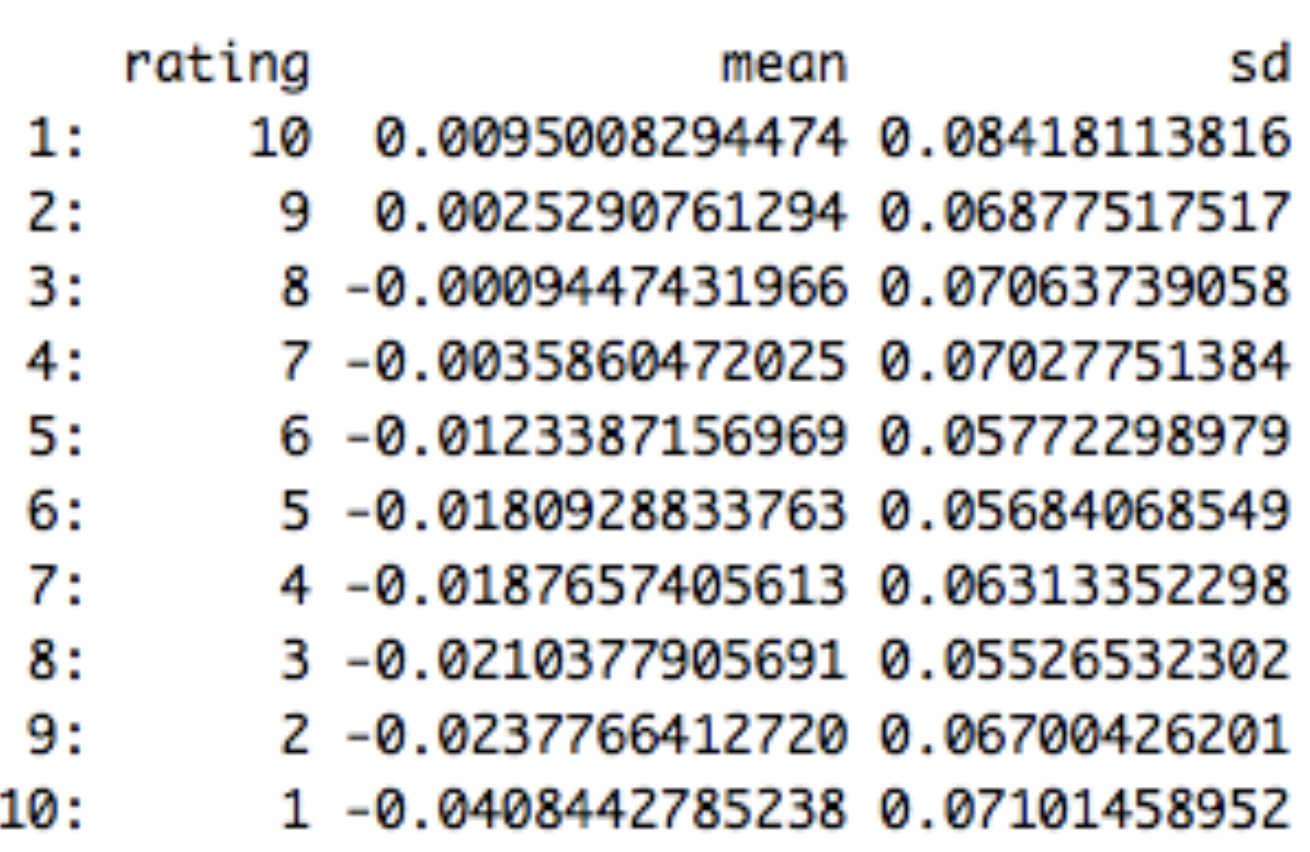
\includegraphics[scale=0.5]{method_and_dicussion_table1.png}
\newline
After further investigation, we discover that the patients
would discuss their pains and describe their disease in the review, in 
which leads to the negative review sentiment score even though the drug’s 
rating is high. Therefore, we need to filter out the negativity brought 
by the condition/disease in order to provide a more accurate result when 
we predict the rating using the review sentiment score. \newline \newline In addition, we notice that some of the ratings get more useful counts 
while others do not. In order to increase our model’s accuracy, we create 
an additional component called useful count ratio, which equals to the 
number of useful count for each individual review/the total number of 
useful counts in the same condition/disease. We believe the reviews 
with more useful counts deserve more weights and modify the getUINN 
function provided by matloff/rectools API to calculate the weighted mean 
sentiment score instead of a simple mean. 

\section{Hypothesis}
\subsection{Linear Model}
Hypothesis: There is a linear relationship between review sentiment score and rating, 
in other words, the verbal reviews are reliable in establishing a numeric 
rating. We assume there is a linear relationship because both of these metrics reflect 
users’ preferences on drugs and measure the same effect. \newline \newline Firstly, we use 
linear regression model to find the review sentiment score’s effect on 
rating:
\[Y_{ij} \sim sentiment\_score + e_{ij}\]
The coefficient for sentiment score equals to 9.88, which indicates the 
linear model considers the review sentiment score has comparatively 
significant effect on the rating. But the Mean Absolute Prediction 
Error (the average of the absolute difference between the prediction 
value and the actual value) is high. 

\section{Latent Factor Model}
Secondly, we use the Latent Factor Model to further investigate the 
linear relationship between the review sentiment score and rating; 
check whether the error rate would decrease. Based on the hypothesis above, 
we can use the review sentiment score to predict rating in the Latent Factor 
Model. If we find the model gives a low Mean Absolute Prediction Error, 
our hypothesis is correct and the linearity between the review sentiment 
score and rating exists. We examine three cases here:
\begin{itemize}
  \item We only include drug’s effect on the mean sentiment score and assume there’s no user IDs.
  \item We include condition/disease and drug’s effect on the mean sentiment score and assume conditionID as userID.
  \item 3)	We include condition/disease and drug’s effect on the mean sentiment score and assume conditionID 
  as userID. In addition, we add more weights to the mean sentiment score that has more useful count.
\end{itemize}
Suppose \(\alpha_i\) = condition i’s effect on the mean sentiment score and
\(\beta_j\) = drug j’s effect on the mean sentiment score. For all the models below, 
we have review\_length as covariate. 
\subsection{Model 1: Includes drug’s effect on the mean sentiment score}
\[E(Y_{ij}|i, j) = u + \beta_j + \epsilon_{ij}\]
The expected numeric rating  =  Prediction from respective overall mean sentiment score of drug j 
\subsection{Model 2: Includes condition and drug’s effect on the mean sentiment score}
\[E(Y_{ij}|i, j) = u + \alpha_i + \beta_j + \epsilon_{ij}\]
The expected numeric rating  = Prediction from respective overall mean sentiment score of condition i and drug j 
\subsection{Model 3: Includes condition and drug’s effect on the mean sentiment score, taking into consideration of the useful count ratio}
\[E(Y_{ij}|i, j) = u + \alpha_i + \beta_j + \epsilon_{ij}\]
with \(\alpha_i\), \(\beta_j\) calculated using weighted mean instead of normal mean
\subsection{Mean Absolute Prediction Error}
We discover that the error rate is the lowest when we add the useful\_count\_ 
ratio/weights to the Latent Factor Model with drug and condition/disease 
effect, followed by the Latent Factor Model with only drug’s effect, 
linear regression model with sentiment score and Latent Factor Model with 
drug and condition effect but without useful\_count\_ratio. However, all the error rates are relatively 
close and large since the rating scale is from 1 to 10. Therefore, we reject our hypothesis based on
the results. The review sentiment score is not reliable in 
establishing the rating, even with the covariates.  \newline

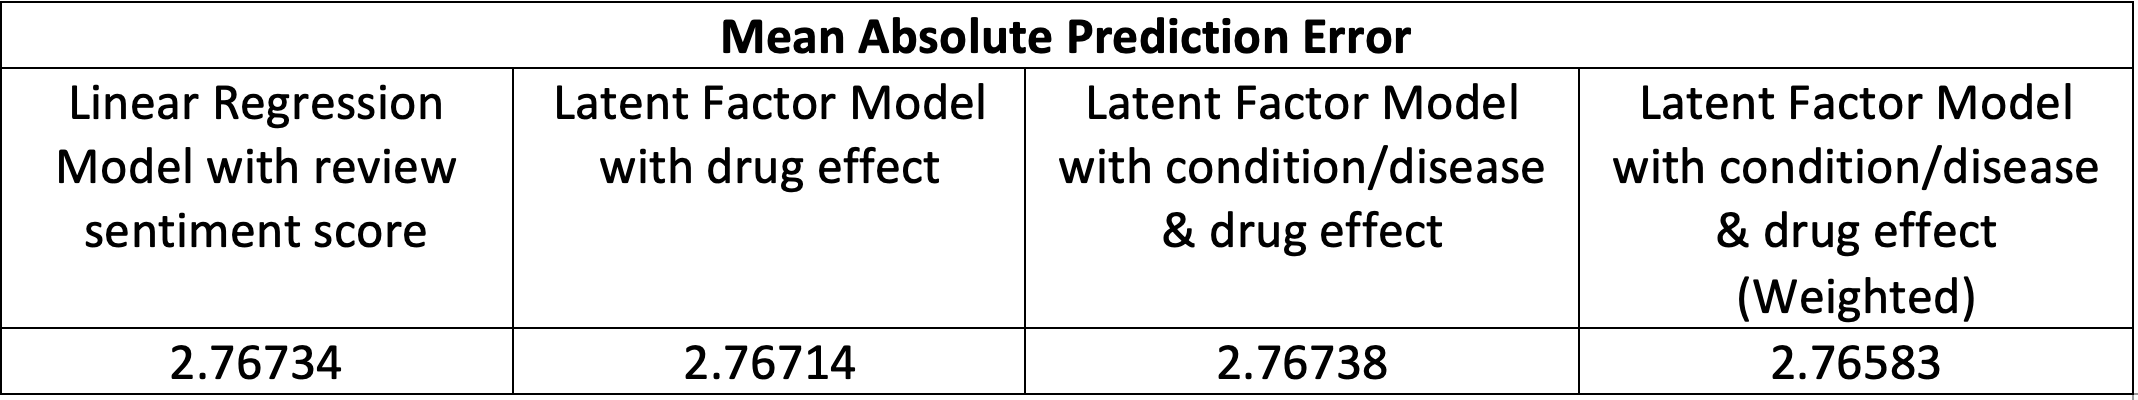
\includegraphics[scale=0.3]{mape_problemB.png}

\section{Neural Network}
We use the neuralnet R package to construct a neural network to predict 
the drug’s rating. The predictive variables are conditionid, 
sentiment\_score, and review\_length. Generally speaking, two layers are 
sufficient to build an effective neural network framework. We then use 
cross validation to find out the optimal number of nodes in the two layers. 
In order for neuralnet to converge, we scale the data and increase the 
stepmax (the maximum steps for the training of the neural network) to 1e8. 
Below is the cross-validation result that we get, and we see that the 
neural network with 5 nodes in layer 1 and 4 nodes in layer 2 has the 
lowest mean absolute prediction error. However, it still performs worse 
than the Latent Factor model. \newline

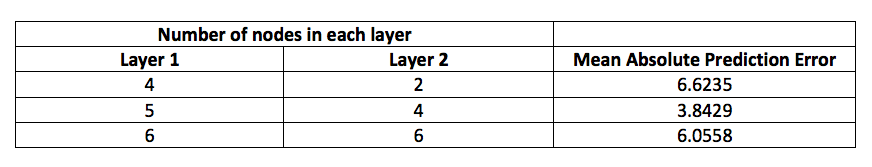
\includegraphics[scale=0.4]{nodes_in_each_layer.jpg}

Below is the neural network graph that shows 
the weights of the best neural network. \newline

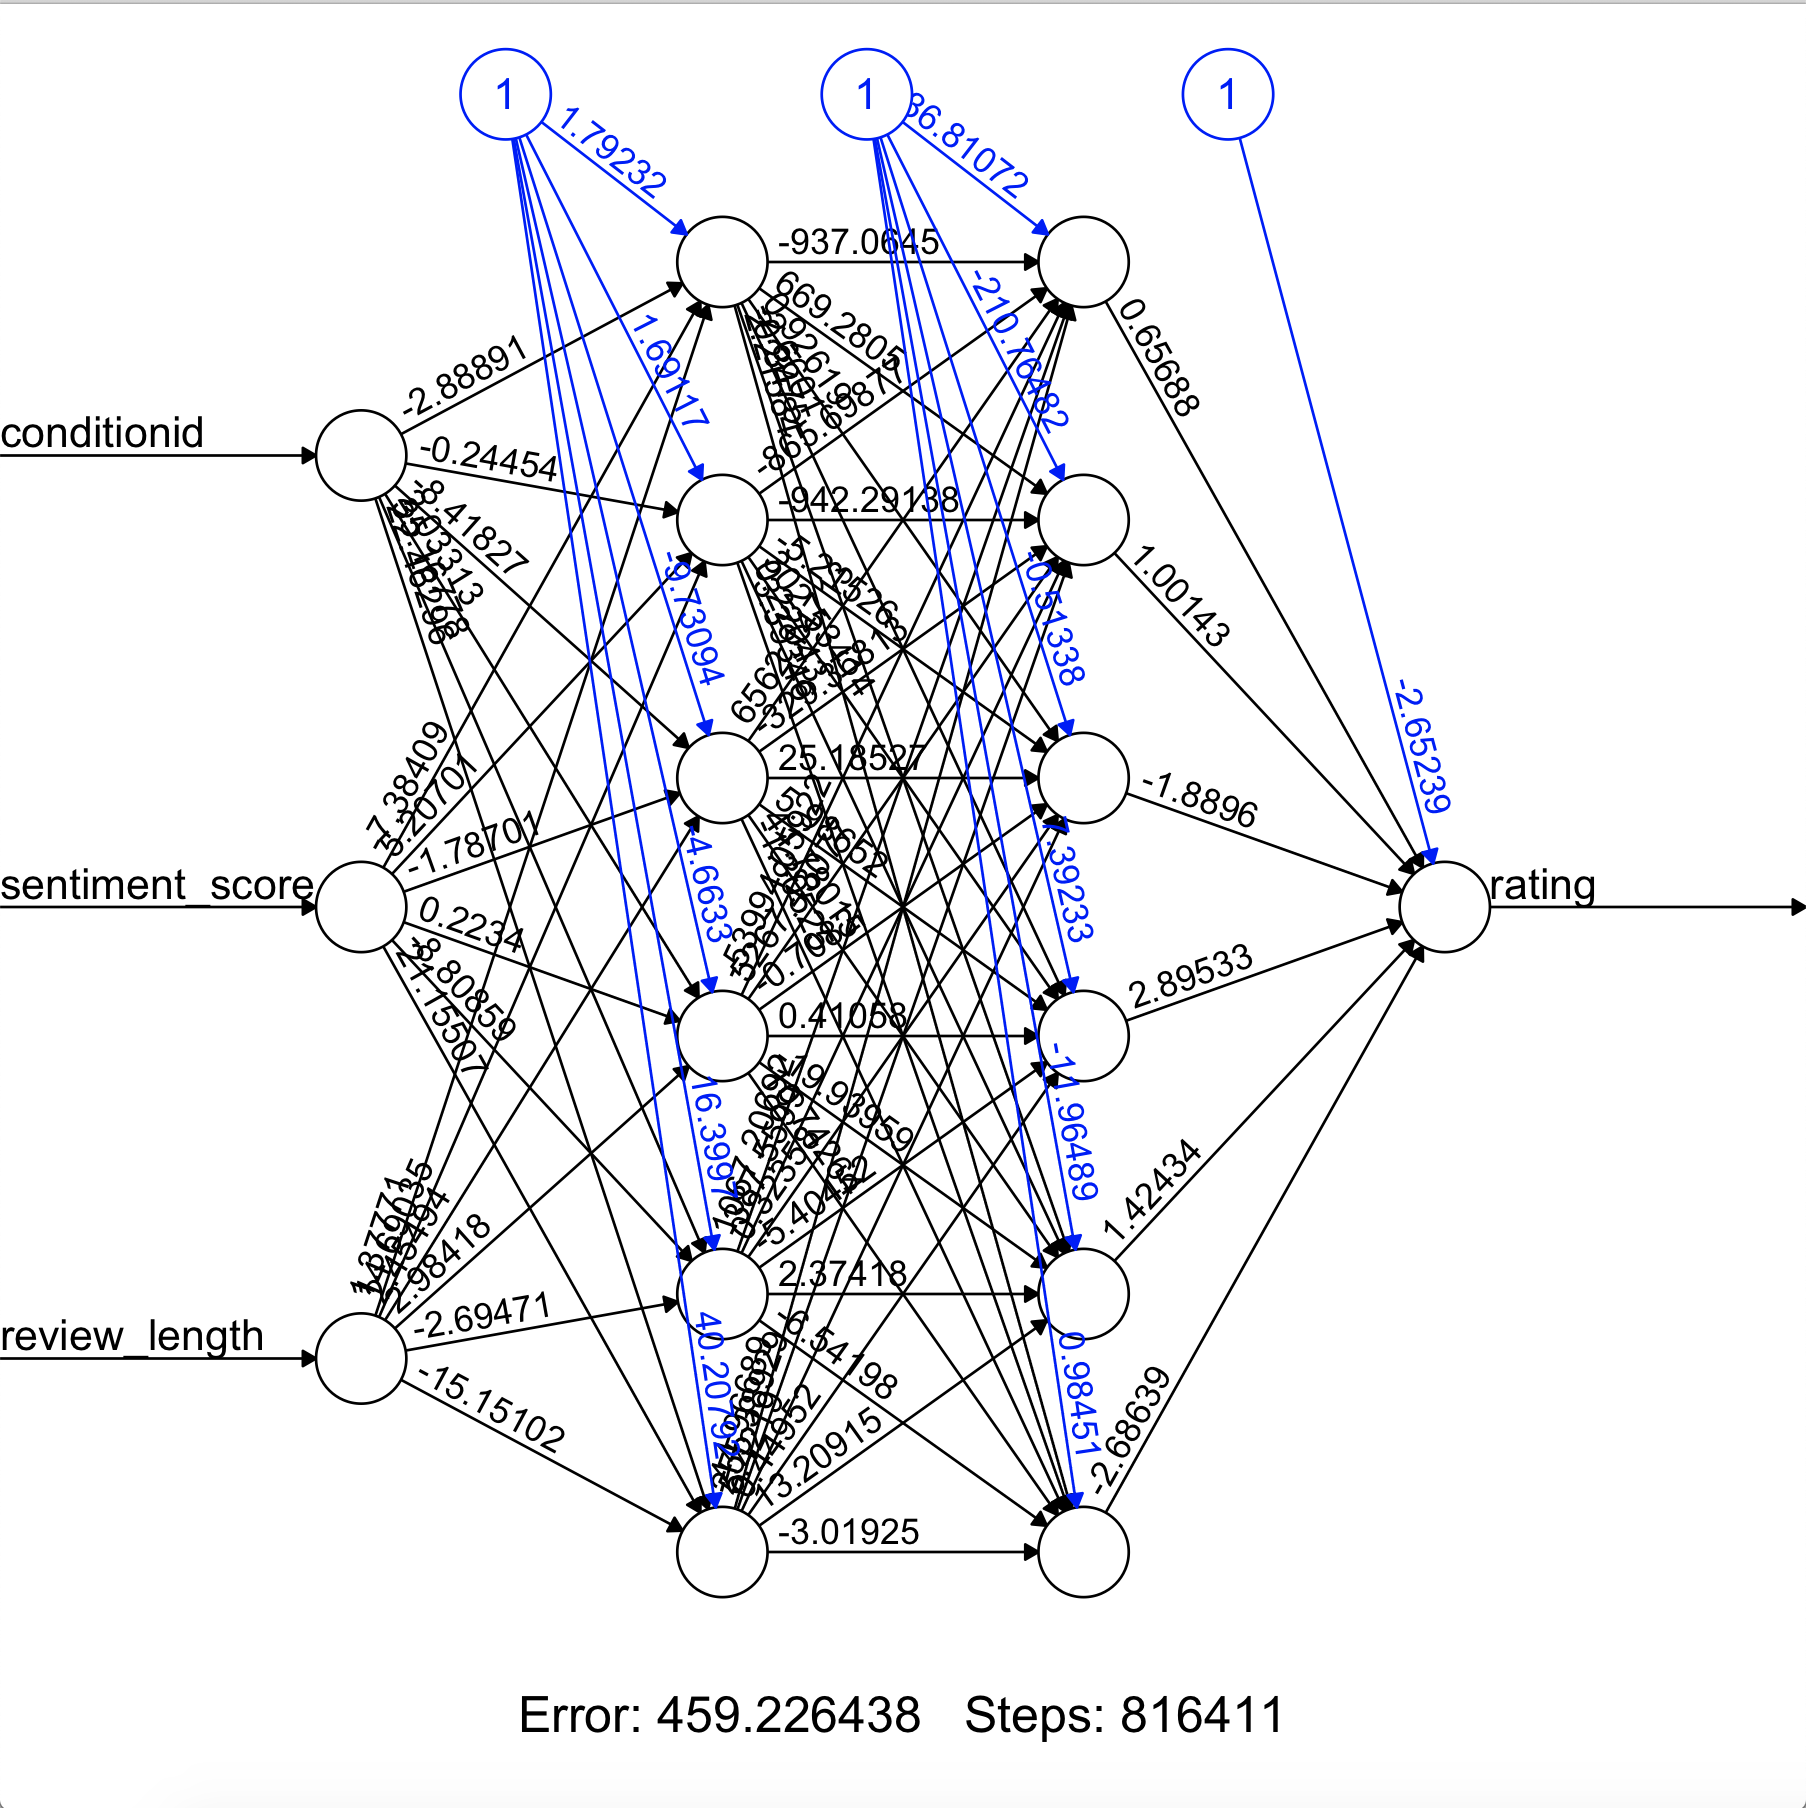
\includegraphics[scale=0.3]{best_neural.png}
\newline
In order to increase the reliability of review sentiment score on the 
numeric rating, we suggest the future researchers to create a 
function/model that separates the review into two parts, one that 
describes the condition/disease and one describes the drug. 
We believe the sentiment score calculated from the drug description 
would be more reliable in getting the actual numeric rating.  

\section{Author Contributions}
All group members contributed equally in this project.

\section{Appendix}
\begin{verbatim}
  # Problem 2
  # 1. drugName (categorical): name of drug 
  # 2. condition (categorical): name of condition 
  # 3. review (text): patient review 
  # 4. rating (numerical): 10 star patient rating 
  # 5. date (date): date of review entry 
  # 6. usefulCount (numerical): number of users who found review useful
  # 
  # train_set(75%), test_set(25%)

  # Use Reference in the Youtube Series created by Data Science Dojo
  # setwd('/Users/jieyichen/Desktop/R Final Project/')
  # linear model and neural networks

  require(data.table)
  drug_test = as.data.frame(fread('drugsComTest_raw.tsv'))
  drug_train = as.data.frame(fread('drugsComTrain_raw.tsv'))

  library(ggplot2)

  data_preprocess = function(dataframe){
    # check whether there are missing values in the data
    if (length(which(!complete.cases(dataframe))) == 0) {
      print('Dataset has no missing values.')
    } else{
      print('Dataset has missing values.')
    }
    print('The table below shows the rating score distribution:')
    # see the rating score distribution
    print(prop.table(table(dataframe$rating)))
    # get the review length
    dataframe$review_length = nchar(dataframe$review)
    return(dataframe)
  }

  ggplot_draw = function(dataframe){
    # visualize the review lengths with class labels
    ggplot(dataframe, aes(x = rating, fill = review_length)) + 
      geom_histogram(bins = 20) + 
      labs(y = 'Review Text Count', x = 'Length of Text', 
      title = 'Distribution of Review Text Lengths with Rating Score') +
      theme(plot.title = element_text(hjust = 0.5))
  }

  drug_train_output = data_preprocess(drug_train)
  ggplot_draw(drug_train_output)
  drug_test_output = data_preprocess(drug_test)
  ggplot_draw(drug_test_output)

  # We have checked that the data distribution is 
  # relatively similar between the train set and test set.


  # Data Pre-Processing Steps:
  # 1) Tokenize the words, remove numbers, punctuations, 
  # symbols and hyphens
  # 2) Covert the case of tokens so that we do not have repetitive words 
  # 3) Filter out the stop words (common words that 
  # provides very little meaning, such as 'the', 'a' and etc)
  # 4) Perform stemming (take similar words and 
  # collapse them into one) on the tokens, 
  # 5) Create a matrix using the pre-processed tokens


  #install.packages('quanteda')
  library(quanteda)

  word_tokenize = function(dataframe) {
    # tokenize the words
    # remove numbers, punctuations, symbols and hyphens 
    # because we only want to analyze the feelings that the 
    # text tries to convey
    dataframe_tokens = tokens(dataframe$review, what = 
    'word', remove_numbers = TRUE, remove_punct = TRUE, 
    remove_symbols = TRUE, remove_hyphens = TRUE)
    # lower case the tokens
    dataframe_tokens = tokens_tolower(dataframe_tokens)
    # remove stop words
    dataframe_tokens = tokens_select(dataframe_tokens, 
    stopwords(), selection = 'remove')
    # stem the tokens
    dataframe_tokens = tokens_wordstem(dataframe_tokens, 
    language = 'english')
    list_text = sapply(dataframe_tokens, as.character)
    return(list_text)
  }

  test_text = word_tokenize(drug_test)
  train_text = word_tokenize(drug_train)

  #install.packages('sentimentr')
  library(sentimentr)

  sentiment_avg = function(text_analyze) {
    # gives a score that indicates the positiveness or 
    # negativeness of the words
    text_sentiment = sentiment(text_analyze)
    # take the average of the sentiment score
    return (mean(text_sentiment$sentiment))
  }

  # We found that the review messages generally converys 
  negative feelings because the patient describes
  # their pains caused by the disease in the review as well. 

  create_feature_df = function(sentiment_score, orig_df) {
    # create sentiment_df with its score
    final_df = data.frame(sentiment_score)
    # select certain columns from df
    orig_df_select = orig_df[, c('drugName', 'condition', 
    'rating', 'usefulCount', 'review_length')]
    # combine sentiment_df with selected_column_df
    drug_df = cbind(final_df, orig_df_select)
    drug_df$drugName = as.numeric(as.factor(drug_df$drugName))
    drug_df$conditionid = as.numeric(as.factor(drug_df$condition))
    drug_df = drug_df[,c('conditionid', 'drugName', 'rating', 
    'sentiment_score', 'usefulCount', 'review_length')]
    return(drug_df)
  }

  mean_rating = function(train_list, drug_train_output){
    train_df = create_feature_df(train_list, drug_train_output)
    # get the mean and sd value
    dt = data.table(train_df)
    dt_table = dt[, list(mean = mean(sentiment_score), sd = 
    sd(sentiment_score)), by = rating]
    
    return (dt_table[with(dt_table, order(-mean))])
  }

  set.seed(9999)
  trainidxs <- sample(1:nrow(drug_train),1200)
  testidxs <- sample(1:nrow(drug_test),400)
  trainset <- drug_train[trainidxs, ]
  testset <- drug_test[testidxs, ]

  train_list = sapply(train_text[trainidxs], sentiment_avg)
  test_list = sapply(test_text[testidxs], sentiment_avg)
  mean_rating(train_list, drug_train_output[trainidxs, ])
  mean_rating(test_list, drug_test_output[testidxs, ])


  library(caret)

  convert_df = function(df_list, drug_train){
    df = create_feature_df(df_list, drug_train)
    # the range of the variable is relatively large, 
    therefore, we need to normalize the data
    # normalize the data in interval [0, 1]
    df$usefulCount = df$usefulCount + 0.1
    
    aggre_sum_condition = aggregate(.~conditionid, df, sum)
    aggre_sum_condition = aggre_sum_condition[, 
    c('conditionid', 'usefulCount')]
    colnames(aggre_sum_condition) = c('conditionid', 
    'usefulCount_condition_sum')
    df = merge(df, aggre_sum_condition, by = 'conditionid', all = T)
    
    aggre_sum_drug = aggregate(.~drugName, df, sum)
    aggre_sum_drug = aggre_sum_drug[, c('drugName', 'usefulCount')]
    
    colnames(aggre_sum_drug) = c('drugName', 'usefulCount_drug_sum')
    
    df = merge(df, aggre_sum_drug, by = 'drugName', all = T)
    
    df$uWeight_condition = df$usefulCount / df$usefulCount_condition_sum
    df$uWeight_drug = df$usefulCount / df$usefulCount_drug_sum
    
    df = df[, c('conditionid',  'drugName',  'rating',  
    'sentiment_score', 'uWeight_condition', 'uWeight_drug', 
    'review_length')]
    
    return(df)
  }


  train_final_df = convert_df(train_list, drug_train_output[trainidxs, ])
  test_final_df = convert_df(test_list, drug_test_output[testidxs, ])


  RStoReg <- function (ratingsIn, useNij = FALSE, weighted = FALSE) 
  {
    UINN <- getUINN(ratingsIn, weighted)
    if (ncol(ratingsIn) > 3) {
      covs <- as.matrix(ratingsIn[, -(1:3)])
      dimnames(covs)[[2]] <- names(ratingsIn[, -(1:3)])
    }
    usrsInput <- as.character(ratingsIn[, 1])
    itmsInput <- as.character(ratingsIn[, 2])
    userMeans <- UINN$uMeans[usrsInput]
    itemMeans <- UINN$iMeans[itmsInput]
    means <- data.frame(uMeans = userMeans, iMeans = itemMeans)
    if (useNij) {
      userN <- UINN$uN[usrsInput]
      itemN <- UINN$iN[itmsInput]
      means <- cbind(means, userN, itemN)
      names(means)[3:4] <- c("uN", "iN")
    }
    if (ncol(ratingsIn) > 3) {
      xy <- cbind(means, covs)
    }
    else xy <- means
    xy <- cbind(xy, ratingsIn[, 3])
    names(xy)[ncol(xy)] <- names(ratingsIn)[3]
    rownames(xy) <- rownames(ratingsIn)
    xy
  }

  getUINN <- function (ratingsIn, weighted = FALSE) 
  {
    users <- as.character(ratingsIn[, 1])
    items <- as.character(ratingsIn[, 2])
    
    if(weighted) {
      ratings1 <- ratingsIn$sentiment_score * ratingsIn$uWeight_condition
      ratings2 <- ratingsIn$sentiment_score * ratingsIn$uWeight_drug
      umean <- function(x) {
        sum(x)
      }
      Ni. <- tapply(ratings1, users, length)
      N.j <- tapply(ratings2, items, length)
      usrMeans <- tapply(ratings1, users, umean)
      itmMeans <- tapply(ratings2, items, umean)
      final <- list(uMeans = usrMeans, iMeans = 
      itmMeans, uN = Ni., iN = N.j)
      return (final)
    } else {
      ratings1 <- ratingsIn$sentiment_score
      ratings2 <- ratingsIn$sentiment_score
      umean <- function(x) {
        mean(x)
      }
      Ni. <- tapply(ratings1, users, length)
      N.j <- tapply(ratings2, items, length)
      usrMeans <- tapply(ratings1, users, umean)
      itmMeans <- tapply(ratings2, items, umean)
      final <- list(uMeans = usrMeans, iMeans = 
      itmMeans, uN = Ni., iN = N.j)
      return (final)
    }
  }


  model_list = list()
  # Linear Model
  # 1)	Yij ~ rev_score + eij
  library(rectools)
  udconv_train = RStoReg(train_final_df, weighted = FALSE)
  # run the linear model
  delete = c('uWeight_condition', 'uWeight_drug')
  udconv_train = udconv_train[, !(colnames(udconv_train) 
  %in% delete), drop=FALSE]
  udconvout = lm(rating ~ ., data = udconv_train[-c(1:2)])
  udconvout$coefficients
  # predict the test_df using the linear model
  udconv_test = RStoReg(test_final_df,weighted = FALSE)
  preds_cov = predict(udconvout, udconv_test)
  model_list[['linear_on_segment_score']] = mean(abs(
    preds_cov - udconv_test[, 'rating']), na.rm = T)


  # 2) E(Yij|i,j) = u + Bj + eij
  udconvout_1 = lm(rating ~ ., data = udconv_train[-1])
  udconvout_1$coefficients
  # predict the test_df using the linear model
  udconv_test_1 = RStoReg(test_final_df,weighted = FALSE)
  preds_cov_1 = predict(udconvout_1, udconv_test_1)
  model_list[['linear_on_imeans']] = mean(abs(preds_cov_1 
  - udconv_test_1[, 'rating']), na.rm = T)

  # 3)	E(Yij|i,j) = u + ai + Bj + eij
  udconvout_2 = lm(rating ~ ., data = udconv_train)
  udconvout_2$coefficients
  # predict the test_df using the linear model
  udconv_test_2 = RStoReg(test_final_df,weighted = FALSE)
  preds_cov_2 = predict(udconvout_2, udconv_test_2)
  model_list[['linear_on_umeans_imeans']] = mean(abs(preds_cov_2 
  - udconv_test_2[, 'rating']), na.rm = T)

  # 4)	E(Yij|i,j) = u + ai + Bj + eij (Weighted)
  udconv_train_3 = RStoReg(train_final_df, weighted = TRUE)
  # run the linear model
  delete = c('uWeight_condition', 'uWeight_drug')
  udconv_train_3 = udconv_train_3[, !(colnames(udconv_train_3) 
  %in% delete), drop=FALSE]
  udconvout_3 = lm(rating ~ ., data = udconv_train_3)
  udconvout_3$coefficients
  # predict the test_df using the linear model
  udconv_test_3 = RStoReg(test_final_df,weighted = TRUE)
  preds_cov_3 = predict(udconvout_3, udconv_test_3)
  model_list[['linear_on_umeans_imeans_weighted']] = 
  mean(abs(preds_cov_3 - udconv_test_3[, 'rating']), na.rm = T)

  model_list


  # Neural Network
  library(neuralnet)

  # scale the data
  scaledData <- scale(train_final_df)

  # get all the column name of the dataframe
  allVars = colnames(train_final_df)
  # remove the "rating", "condition_id", "drugName" 
  # from all vars and the rest are predictor variables
  predictorVars = allVars[!allVars%in% c("rating", 
  "condition_id", "drugName", "uWeight_condition", "uWeight_drug")]

  predictorVars = paste(predictorVars, collapse = "+")
  form = as.formula(paste("rating~", predictorVars, collapse = "+"))

  # 4 hidden nodes in the second layer and 2 hidden nodes 
  # in the third layer

  neuralnet_cv = function(node_layer_1, node_layer_2){
    neuralModel = neuralnet(formula = form, hidden = 
    c(node_layer_1, node_layer_2), linear.output = TRUE, 
    data = scaledData, stepmax=1e8)
    plot(neuralModel)
    # Neural network produces continuous variable 
    # because our last layer uses linear output. 
    predictions = compute(neuralModel, test_final_df[, 
    allVars[!allVars%in%c("rating", "condition_id", 
    "drugName", "uWeight_condition", "uWeight_drug")]])
    scaledResults = predictions$net.result * attr(scaledData, 
    "scaled:scale")["rating"]  + attr(scaledData, 
    "scaled:center")["rating"]
    return(mean(abs(scaledResults - udconv_test[, 'rating'])))
  }

  # do cross validation to find the optimal hidden nodes 
  # for the neural network
  hidden_node_df = data.frame(c(4, 2), c(5, 4), c(6, 6))
  hidden_node_df = data.frame(t(hidden_node_df))
  names(hidden_node_df) = c('nodes_layer_1', 'nodes_layer_2')

  for (num_row in seq(1, nrow(hidden_node_df))) {
    node_layer_1 = hidden_node_df$nodes_layer_1[num_row]
    node_layer_2 = hidden_node_df$nodes_layer_2[num_row]
    hidden_node_df$error_rate[num_row] = 
    c(neuralnet_cv(node_layer_1, node_layer_2))
  }

  rownames(hidden_node_df) = NULL
  hidden_node_df
\end{verbatim}

\begin{thebibliography}{1}

  \bibitem{rsbook} Norman Matloff {\em A Tour of Recommender Systems}  2018.
  \bibitem{TextAnalyticsYoutube} Data Science Dojo (Youtube) {\em Introduction to Text Analytics with R: Data Pipelines}  2017.
  \bibitem{NeuralNetworksYoutube} Data Science by Arpan Gupta IIT, Roorkee (Youtube) {\em Neural Networks in R}  2017.
  
\end{thebibliography}

\end{document}